\documentclass{beamer}

%%%%%%%%%%%%%%%%%%%%%%%%%%%%%%%%%%%%%%%
%   Language abstraction commands     %
%%%%%%%%%%%%%%%%%%%%%%%%%%%%%%%%%%%%%%%

% spacing
\newcommand{\gap}{\quad\quad}
\newcommand{\biggap}{\quad\quad\quad}
\newcommand{\nextline}{\\ \\}
\newcommand{\htabwidth}{0.5cm}
\newcommand{\tabwidth}{1cm}
\newcommand{\htab}{\hspace{\htabwidth}}
\newcommand{\tab}{\hspace{\tabwidth}}
\newcommand{\linesep}{\ \hrulefill \ \smallskip}

\newcommand{\mi}[1]{\mathit{#1}}

% misc symbols
\newcommand{\dhd}{\!\!\!\!\!\rightarrow}
\newcommand{\Dhd}{\!\!\!\!\!\Rightarrow}
\newcommand{\ts}{\,\vdash\,}
\newcommand{\la}{\langle}
\newcommand{\ra}{\rangle}
\newcommand{\eg}{{\em e.g.}}

% misc identifiers
\newcommand{\dom}{\mbox{\sl dom}}
\newcommand{\fn}{\mbox{\sl fn}}
\newcommand{\bn}{\mbox{\sl bn}}
\newcommand{\sig}{\mbox{\sl sig}}
\newcommand{\IF}{\mbox{\mathem if}}
\newcommand{\OTHERWISE}{\mbox{\mathem otherwise}}
\newcommand{\expand}{\prec}
\newcommand{\weakexpand}{\prec^W}
\newcommand{\spcomma}{~,~}

%% Relations
% Subtype 
\newcommand{\sub}{<:}
% Type assignment
\newcommand{\typ}{:}
% reduction
\newcommand{\reduces}{\;\rightarrow\;}
% well-formedness
\newcommand{\wf}{\;\mbox{\textbf{wf}}}
\newcommand{\nswf}{\mbox{\textbf{wf}}}
\newcommand{\wfe}{\;\mbox{\textbf{wfe}}}
\newcommand{\nswfe}{\mbox{\textbf{wfe}}}

%% Operators
% Type selection
\newcommand{\tsel}{\#}
% Function type
\newcommand{\tfun}{\rightarrow}
\newcommand{\dfun}[3]{(#1\!:\!#2) \Rightarrow #3}
% Conjunction
\newcommand{\tand}{\wedge}
% Disjunction
\newcommand{\tor}{\vee}
% Singleton type suffix
\newcommand{\sing}{.\textbf{type}}

%% Syntax
% Header for typing rules
\newcommand{\judgement}[2]{{\bf #1} \hfill #2}
% Widening
\newcommand{\wid}[2]{#1 : #2}
% Refinement
\newcommand{\refine}[2]{\left\{#1 \Rightarrow #2 \right\}}
\newcommand{\mlrefine}[2]{\{#1 \Rightarrow #2 \}}
% Field definitions
\newcommand{\ldefs}[1]{\left\{#1\right\}}
\newcommand{\mlldefs}[1]{\{#1\}}
% Member sequences
\newcommand{\seq}[1]{\overline{#1}}
% Lambda
\newcommand{\dabs}[3]{(#1\!:\!#2)\Rightarrow #3}
\newcommand{\abs}[3]{\lambda #1\!:\!#2.#3}
% Method Application
\newcommand{\mapp}[3]{#1.#2(#3)}
% Substitution
\newcommand{\subst}[3]{[#1/#2]#3}
% Object creation
\newcommand{\new}[3]{\textbf{val }#1 = \textbf{new }#2 ;\; #3}
\newcommand{\mlnew}[3]{\textbf{val }#1 = \textbf{new }#2 ;\;\\&#3}
%\renewcommand{\new}[3]{#1 \leftarrow #2 \,\textbf{in}\, #3}
% Field declaration
\newcommand{\Ldecl}[3]{#1 : #2..#3}%{#1 \operatorname{>:} #2 \operatorname{<:} #3}
\newcommand{\ldecl}[2]{#1 : #2}
\newcommand{\mdecl}[3]{#1 : #2 \tfun #3}
% Top and Bottom
\newcommand{\Top}{\top}%{\textbf{Top}}
\newcommand{\Bot}{\bot}%\textbf{Bot}}
% Environment extension
%\newcommand{\envplus}[1]{\uplus \{ #1 \}}
\newcommand{\envplus}[1]{, #1}
% Reduction
\newcommand{\reduction}[4]{#1 \operatorname{|} #2 \reduces #3 \operatorname{|} #4}

% Sugar
\newcommand{\arrow}[2]{#1\rightarrow_s#2}
\newcommand{\fun}[4]{\textbf{fun } (#1:#2)\;#3\;#4}
\newcommand{\app}[2]{(\textbf{app }#1\;#2)}
\newcommand{\mlapp}[2]{(\textbf{app }#1\;\\&#2)}
\newcommand{\cast}[2]{(\textbf{cast }#1\;#2)}

\newcommand{\lindent}{\hspace{-4mm}}

% Logical relations
\newcommand{\relv}[4]{\mathcal{V}_{#1;#2;#3}\llbracket#4\rrbracket}
\newcommand{\rele}[4]{\mathcal{E}_{#1;#2;#3}\llbracket#4\rrbracket}
\newcommand{\rels}[3]{\mathcal{\supseteq}_{#1}\llbracket#2;#3\rrbracket}
\newcommand{\relg}[3]{\mathcal{\supseteq^!}_{#1;#2}\llbracket#3\rrbracket}
\newcommand{\irred}[2]{\text{irred }(#1,#2)}
\newcommand{\andl}{\;\wedge\;}
\newcommand{\orl}{\vee}
\newcommand{\impliesl}{\rightarrow}
\newcommand{\reductionl}[5]{#1 \operatorname{|} #2 \;\rightarrow^{#5}\; #3 \operatorname{|} #4}
\newcommand{\ds}{\,\vDash\,}

\usepackage{bcprules}
\usepackage{multicol}

\usepackage{minted}
\usemintedstyle{eclipse}
% I added & and | as Scala keywords in Pygments:
%% diff -r 121c75491e0d pygments/lexers/jvm.py
%% --- a/pygments/lexers/jvm.py	Tue May 06 20:21:16 2014 -0700
%% +++ b/pygments/lexers/jvm.py	Sat May 10 19:21:51 2014 +0200
%% @@ -259,7 +259,7 @@
%%               u'lazy|match|new|override|pr(?:ivate|otected)'
%%               u'|re(?:quires|turn)|s(?:ealed|uper)|'
%%               u't(?:h(?:is|row)|ry)|va[lr]|w(?:hile|ith)|yield)\\b|'
%% -             u'(<[%:-]|=>|>:|[#=@_\u21D2\u2190])(\\b|(?=\\s)|$)', Keyword),
%% +             u'(<[%:-]|\\&|(\\|)|=>|>:|[#=@_\u21D2\u2190])(\\b|(?=\\s)|$)', Keyword),
%%              (u':(?!%s)' % op, Keyword, 'type'),
%%              (u'%s%s\\b' % (upper, idrest), Name.Class),
%%              (r'(true|false|null)\b', Keyword.Constant),


\usepackage{verbatim}
\usepackage{hyperref}

\useoutertheme{infolines}
\setbeamertemplate{headline}{}
\setbeamertemplate{footline}{
  \hfill
  \usebeamercolor[fg]{page number in head/foot}
  \usebeamerfont{page number in head/foot}
  \insertpagenumber\kern1em\vskip10pt
}
\setbeamertemplate{navigation symbols}{}

\title{Foundations of Path-Dependent Types}
%\subtitle{({\bf D}ependent {\bf O}bject {\bf T}ypes)}
\author{Nada Amin, {\it Tiark Rompf}, Martin Odersky}
\institute{OOPSLA}
\date{October 23, 2014}

\AtBeginSection{
  \begin{frame}
    \begin{center}
      \structure{\Huge \insertsection}
    \end{center}
  \end{frame}
}

\begin{document}

\frame{\titlepage}

\begin{frame}[fragile]

\includegraphics[width=\textwidth]{industry.png}
\end{frame}

\begin{frame}[fragile]
\begin{itemize}
\item Formal description of the Scala type system?
\item Type soundness proof?
\end{itemize}
\end{frame}


\begin{frame}[fragile]{People have tried ...}
\begin{itemize}
\item 2003: $\nu$Obj
\item 2006: Featherweight Scala
\item 2008: Scalina
\item 2008-2010: ScalaClassic
\item 2011-now: DOT (Dependent Object Types)
\end{itemize}
No mechanized soundness proof.
\end{frame}


\begin{frame}[fragile]{Why is it so hard?}
\begin{itemize}
\item Scala is a rich language
\item We haven't fully understood some of its core features
\item Maybe we aren't doing this right ...
\end{itemize}
\end{frame}


\begin{frame}[fragile]{In this paper:}
\begin{itemize}
\item Bottom up instead of top down
\item Focus only on the core: \\
path-dependent types and objects with type members
\item Mechanized soundness proof!
\item Valuable insights into why extending the system is hard
\end{itemize}
\end{frame}



%%%%%  intro DOT / Scala


\section{Types in Scala and DOT}


\begin{frame}[fragile]{DOT: Dependent Object Types}
\begin{itemize}
\item DOT is a core calculus for path-dependent types.
\item Aim: simplify Scala's type system and make it more regular.
\end{itemize}
\end{frame}



\begin{frame}[fragile]{Types in Scala}
\begin{description}[functional]
\item[`modular']\begin{description}[higher-kinded types]
\item[named type]\mint{scala}|scala.collection.BitSet|
\item[compound type]\mint{scala}|Channel with Logged|
\item[refined type]\mint{scala}|Channel { def close(): Unit } |
\end{description}
\item[`functional']\begin{description}[higher-kinded types]
\item[parameterized type]\mint{scala}|List[String]|
\item[existential type]\mint{scala}|List[T] forSome { type T }|
\item[higher-kinded type]\mint{scala}|List|
\end{description}
\end{description}
\begin{comment}
too many orthogonal concepts?
can we simplify by keeping only the modular features?
\end{comment}
\end{frame}



\begin{frame}[fragile]{Reducing Functional to Modular?}
\begin{itemize}
\item type parameter to type member\\
\mint{scala}|class List[Elem] {} /*vs*/ class List { type Elem }|
\item parameterized type to refined type\\
\mint{scala}|List[String] /*vs*/ List { type Elem = String }|
\item existential type?\\
\mint{scala}|List[T] forSome { type T } /*vs*/ List|
\item higher-kinded type?\\
\mint{scala}|List /*vs*/ List|
\end{itemize}
\end{frame}


\begin{frame}[fragile]{Types in DOT}
\begin{description}[declarations]
\item[types]\mint{scala}|S, T, U|
\begin{description}[path-dependent type]
\item[path-dependent type]\mint{scala}|p.L|
\item[refined type]\mint{scala}|T { z => D }|
\item[intersection]\mint{scala}|T & T|
\item[union]
\begin{minted}{scala}
T | T
\end{minted}
\item[top]\mint{scala}|Any|
\item[bottom]\mint{scala}|Nothing|
\end{description}
\item[declarations]\mint{scala}|D|
\begin{description}[path-dependent type]
\item[type declaration]\mint{scala}|type L >: S <: U|
\item[field declaration]\mint{scala}|val l: U|
\item[method declaration]\mint{scala}|def m(x: S): U|
\end{description}
\end{description}
\end{frame}



%%%%% µDOT?

\section{$\mu$DOT}


\begin{frame}[fragile]{${\mu}${DOT}$_T$: Syntax of Types}

$\begin{array}{ll}
x, y, z & \mbox{Variable} \\
S, U, T ::= & \mbox{Type} \\
\gap  \tbnd{z}{\seq{D}} & \mbox{Record Type} \\
\gap  x.L & \mbox{Type Selection} \\
D ::= & \mbox{Member Declaration}\\
\gap  \tmem{L}{S}{U} & \mbox{Type Member}\\
\gap  \tmemup{L}{U}    & \mbox{Type Member (Upper-Bounded)}
\end{array}$

\end{frame}


\begin{frame}[fragile]{Path-Dependent Types: Example}
\begin{minted}{scala}
trait Animal { type Food; def gets: Food
               def eats(food: Food) {}; }
trait Grass; trait Meat
trait Cow extends Animal with Meat {
  type Food = Grass; def gets = new Grass {} }
trait Lion extends Animal {
  type Food = Meat;  def gets = new Meat {} }
val leo = new Lion {}
val milka = new Cow {}
leo.eats(milka) // ok
val lambda: Animal = milka
lambda.eats(milka) // type mismatch
// found : Cow
// required: lambda.Food
lambda.eats(lambda.gets) // ok
\end{minted}
\end{frame}


\begin{frame}[fragile]{Path-Dependent Types: Example}
\begin{minted}{scala}
type Meat = {                    def newMeat  = new {
  type IsMeat = Any }              type IsMeat = Any  }
type Grass = {                   def newGrass = new {
  type IsGrass = Any }             type IsGrass = Any  }
type Animal = { a =>             def newCow   = new {
  type Food                        type IsMeat = Any
  def eats(food: a.Food): Unit     type Food = Grass
  def gets: a.Food                 def eats(food: Grass) = ()
}                                  def gets = newGrass
type Cow = {                     }
  type IsMeat = Any              def newLion = new {
  type Food <: Grass               type Food = Meat
  def eats(food: Grass): Unit      def eats(food: Meat) = ()
  def gets: Grass }                def gets = newMeat }
type Lion = {
  type Food = Meat               val milka = newCow
  def eats(food: Meat): Unit     val leo = newLion
  def gets: Meat }               leo.eats(milka)
\end{minted}
\end{frame}




\begin{frame}[fragile]%{${\mu}${DOT}$_T$: Semantics of Types}

\begin{multicols}{2}[\judgement{Subtyping of Types}{\fbox{$\Gamma \ts S \sub U$}}]
\end{multicols}

\infrule[\textsc{$\sub$-tsel}]
{\Gamma \ts x \ni \tmem{L}{S}{U} \spcomma S' \sub S \spcomma S \sub U}
{\Gamma \ts S' \sub x.L}

\infrule[\textsc{tsel-$\sub$}]
{\Gamma \ts x \ni \tmem{L}{S}{U} \spcomma U \sub U' \spcomma S \sub U}
{\Gamma \ts x.L \sub U'}

\infrule[\textsc{rec-$\sub$-rec}]
{\Gamma \envplus{z: \tbnd{z}{\seq{D}}} \ts \seq{D} \sub \seq{D'}}
{\Gamma \ts \tbnd{z}{\seq{D}} \sub \tbnd{z}{\seq{D'}}}

\begin{multicols}{2}[\judgement{Subtyping of Declarations}{\fbox{$\Gamma \ts D \sub D'$}}]
\end{multicols}

\infrule[\textsc{tdecl-$\sub$-tdecl}]
{\Gamma \ts S' \sub S \spcomma U \sub U'\\
 \Gamma \ts S \sub U \spcomma S'\sub  U'}
{\Gamma \ts (\tmem{L}{S}{U}) \sub (\tmem{L}{S'}{U'})}

\end{frame}


%%%%% Transitivity and Narrowing

\section{Challenges: Transitivity, Narrowing, Inversion}

\begin{frame}[fragile]{Transitivity, Narrowing}

\infrule[\textsc{$\sub$-narrow}]
{\Gamma^a , (x: U) , \Gamma^b \ts T \sub T'\\
 \Gamma^a \ts S \sub U}
{\Gamma^a , (x: S) , \Gamma^b \ts T \sub T'}

\infrule[\textsc{$\sub$-trans}]
{\Gamma \ts S \sub T \spcomma T \sub U}
{\Gamma \ts S \sub U}

\end{frame}

\begin{frame}[fragile]{Solution Attemps}
\begin{itemize}
\item Attempt 0: independent proofs -- clearly doesn't work
\item Attempt 1: induction on subtyping derivation\\problem: contravariant positions
\item Attempt 2: induction on middle type in $T_1 \sub T_2 \sub T_3$ (like F$_{\sub}$)\\problem: $T_1 \sub p.L \sub T_2$
\item Attempt 3: induction on a well-formedness witness\\problem: cyclicity
\item Attempt 4: add transitivity axiom\\problem: inversion lemma
\item Solution: transitivity axiom plus ``push-back'': eliminate 
uses of axiom after the fact
\end{itemize}
\end{frame}



\section{Challenge: Type Preservation}
\begin{frame}[fragile]{Type Preservation}
\begin{minted}{scala}
trait Brand {
  type Hidden
  def pack(x: Int): Hidden
  def unpack(x: Hidden): Int
}
val brand: Brand = new Brand {
  type Hidden = Int
  def pack(x: Int): Hidden = x
  def unpack(x: Hidden): Int = x
}
brand.unpack(brand.pack(7)) // ok
brand.unpack(7) // not ok -- but occurs during reduction!
\end{minted}
\begin{itemize}
\item Solution: big-step semantics with step-index
\item Work with types from the original program instead of re-assigning types to partially evaluated terms
\end{itemize}
\end{frame}




%%%%% Extending to full DOT?

\section{Extending to full DOT?}

\begin{frame}[fragile]{Adding a bottom type breaks}
Type $\Bot$ is a subtype of all other types, including \mint{scala}|{ type E = Int }| 
and \mint{scala}|{ type E = String }|.

So if p: $\Bot$ we have Int $<:$ p.E and p.E $<:$ String. 

Transitivity would give us Int $<:$ p.E $<:$ String!

Subtyping lattice collapses.

\vspace{1em}
Adding intersection types is equivalent to bottom (bad bounds!)

\end{frame}


\begin{frame}[fragile]{Observations and Ideas}
\begin{itemize}
\item Bottom types do not occur at runtime!
\item Is it enough to have transitivity and narrowing in ``realizable'' environments?
\item Have a (restrictive) static type system and a (lenient) one during evaluation
\end{itemize}
\end{frame}



%%%%% The End

\section{Thank you!}

% oopsla14.namin.net




%%%%% Type Inference

\section{Type Inference}

\begin{frame}[fragile]{Type Inference in Scala (Least Upper Bound?)}
\begin{minted}{scala}
trait A { type T <: A }
trait B { type T <: B }
trait C extends A with B { type T <: C }
trait D extends A with B { type T <: D }
// in Scala, lub(C, D) is an infinite sequence
A with B { type T <: A with B { type T <: ... } }

// in Scala REPL
> val o = if (true) (new C{}) else (new D{})
o: A with B{type T <: A with B} = ...
> val o:A with B{type T<:A with B {type T<:A with B}} =
          if (true) (new C{}) else (new D{})
o: A with B{type T <: A with B{type T <: A with B}} = ...
\end{minted}
\end{frame}

\begin{frame}[fragile]{Type Inference in Scala (Working too Hard too Soon?)}
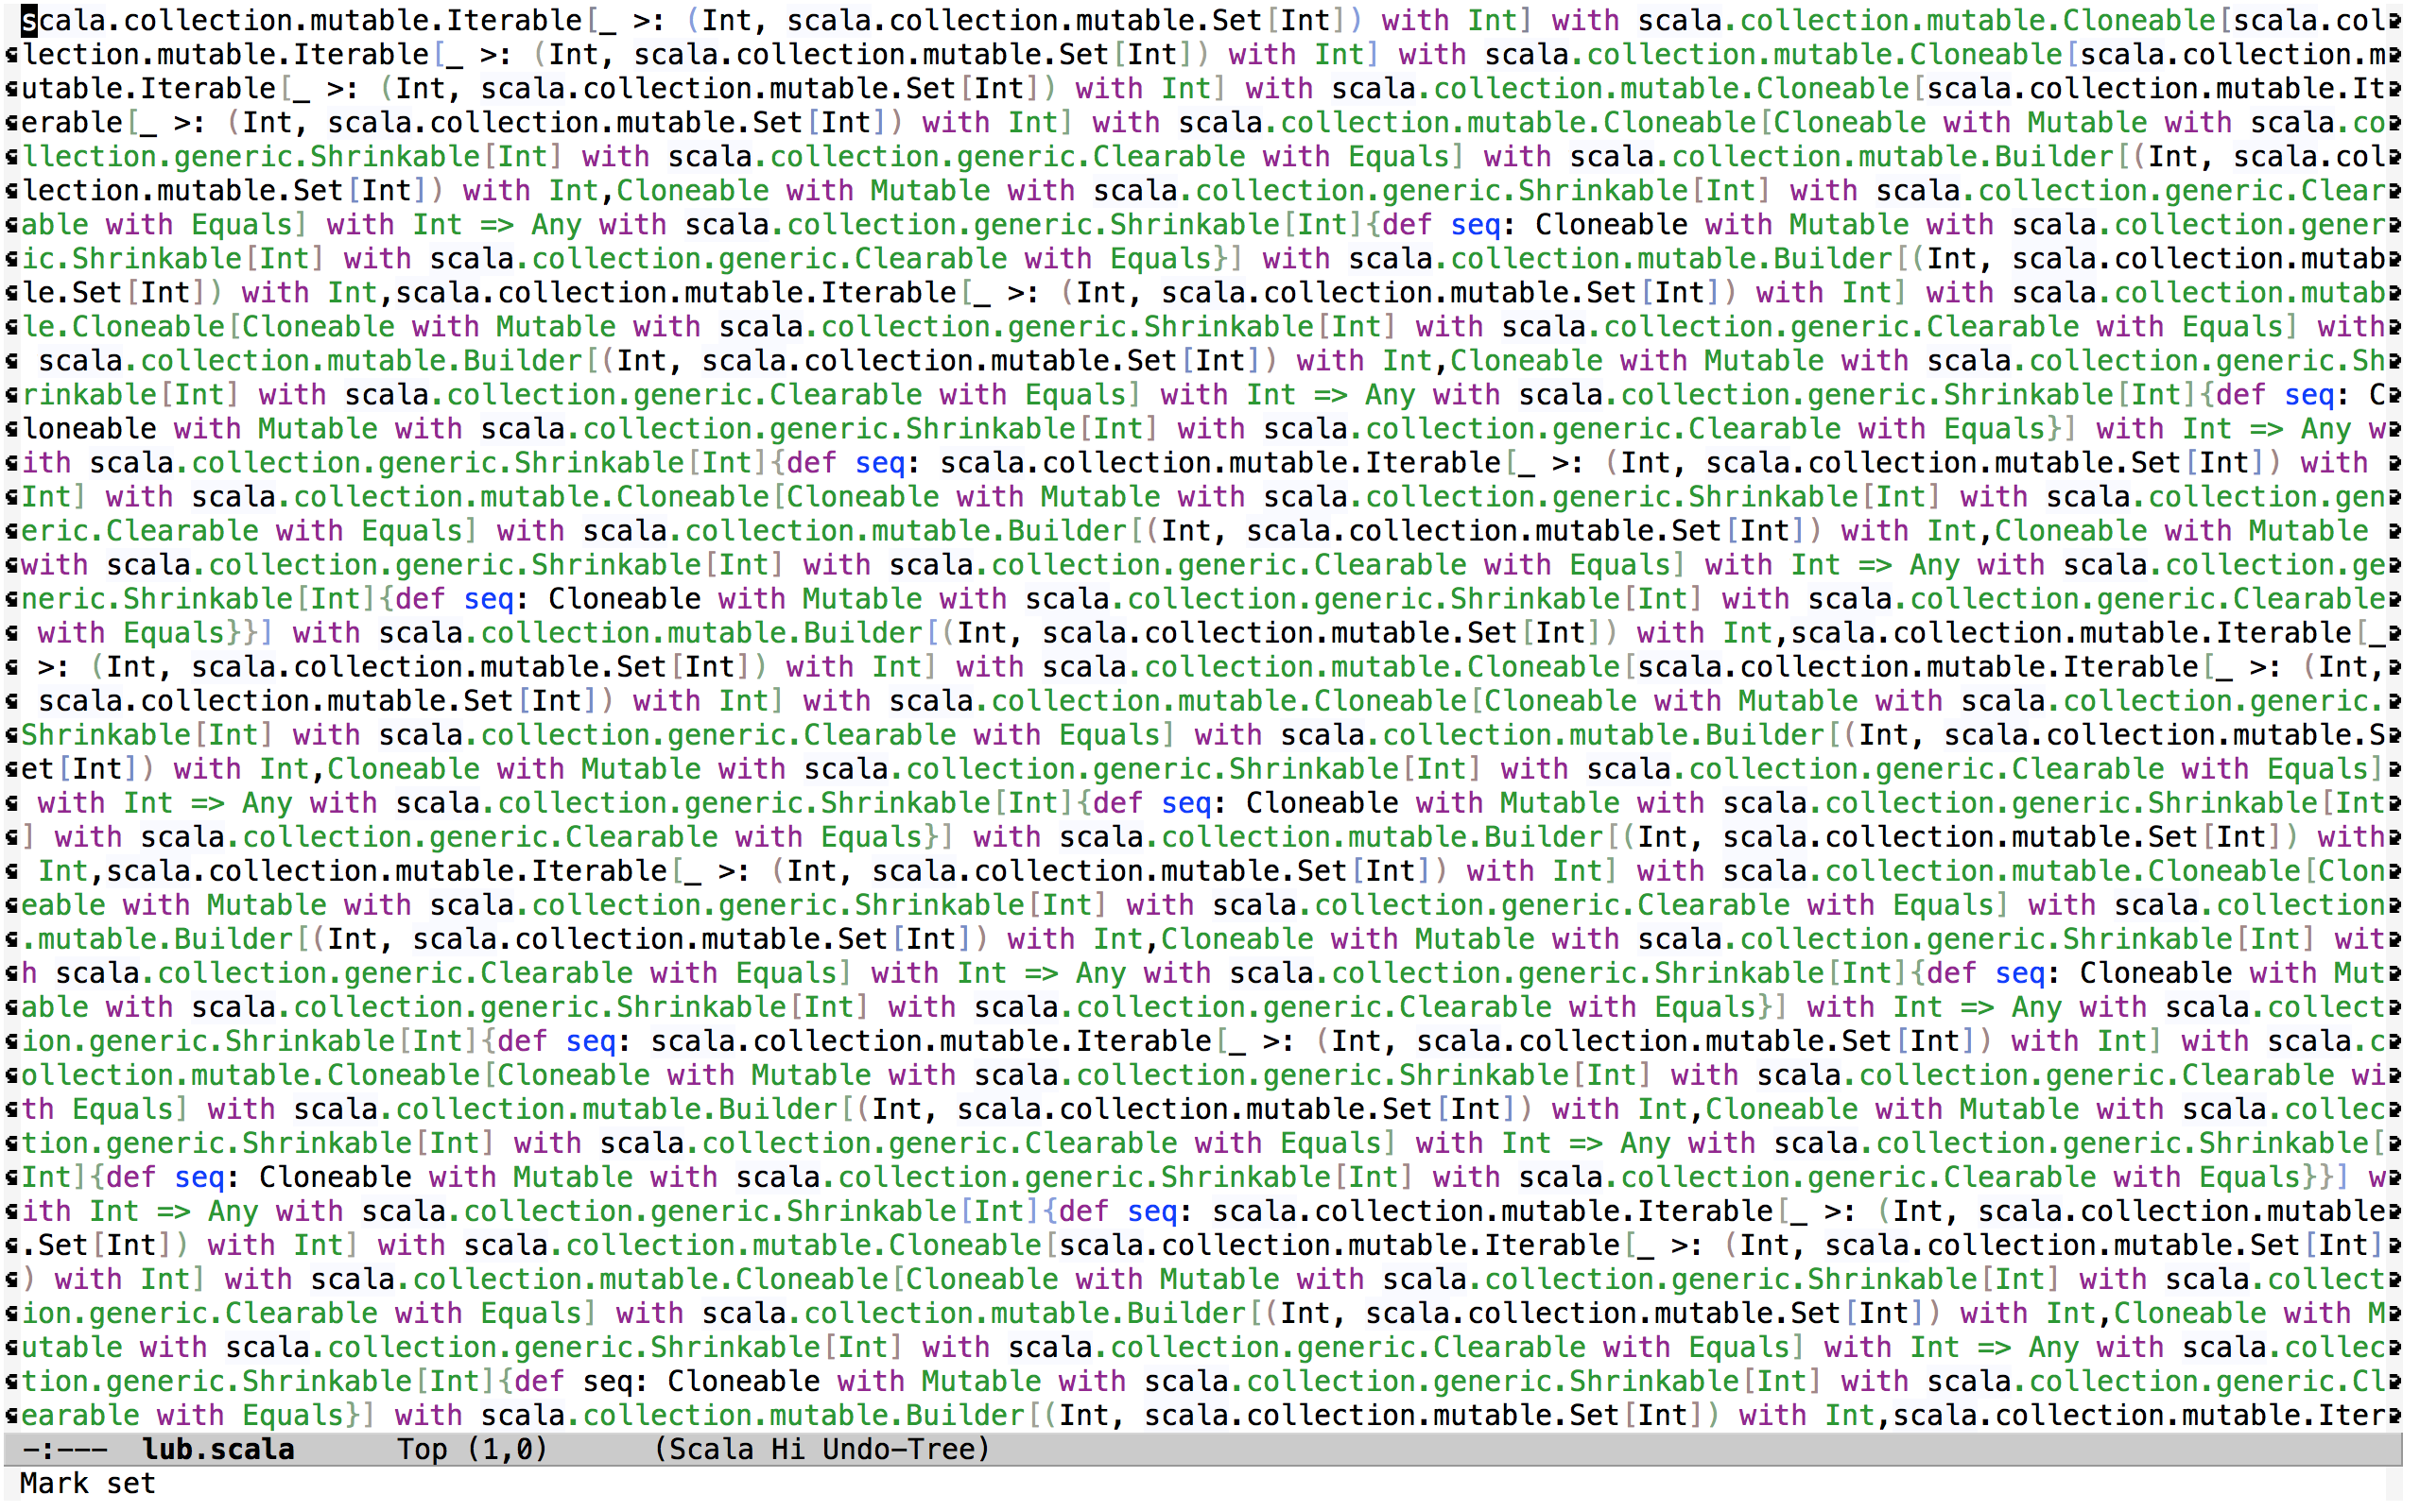
\includegraphics[width=\textwidth]{lub1.png}
\end{frame}

\begin{frame}[fragile]{Type Inference in Scala (Working too Hard too Soon?)}
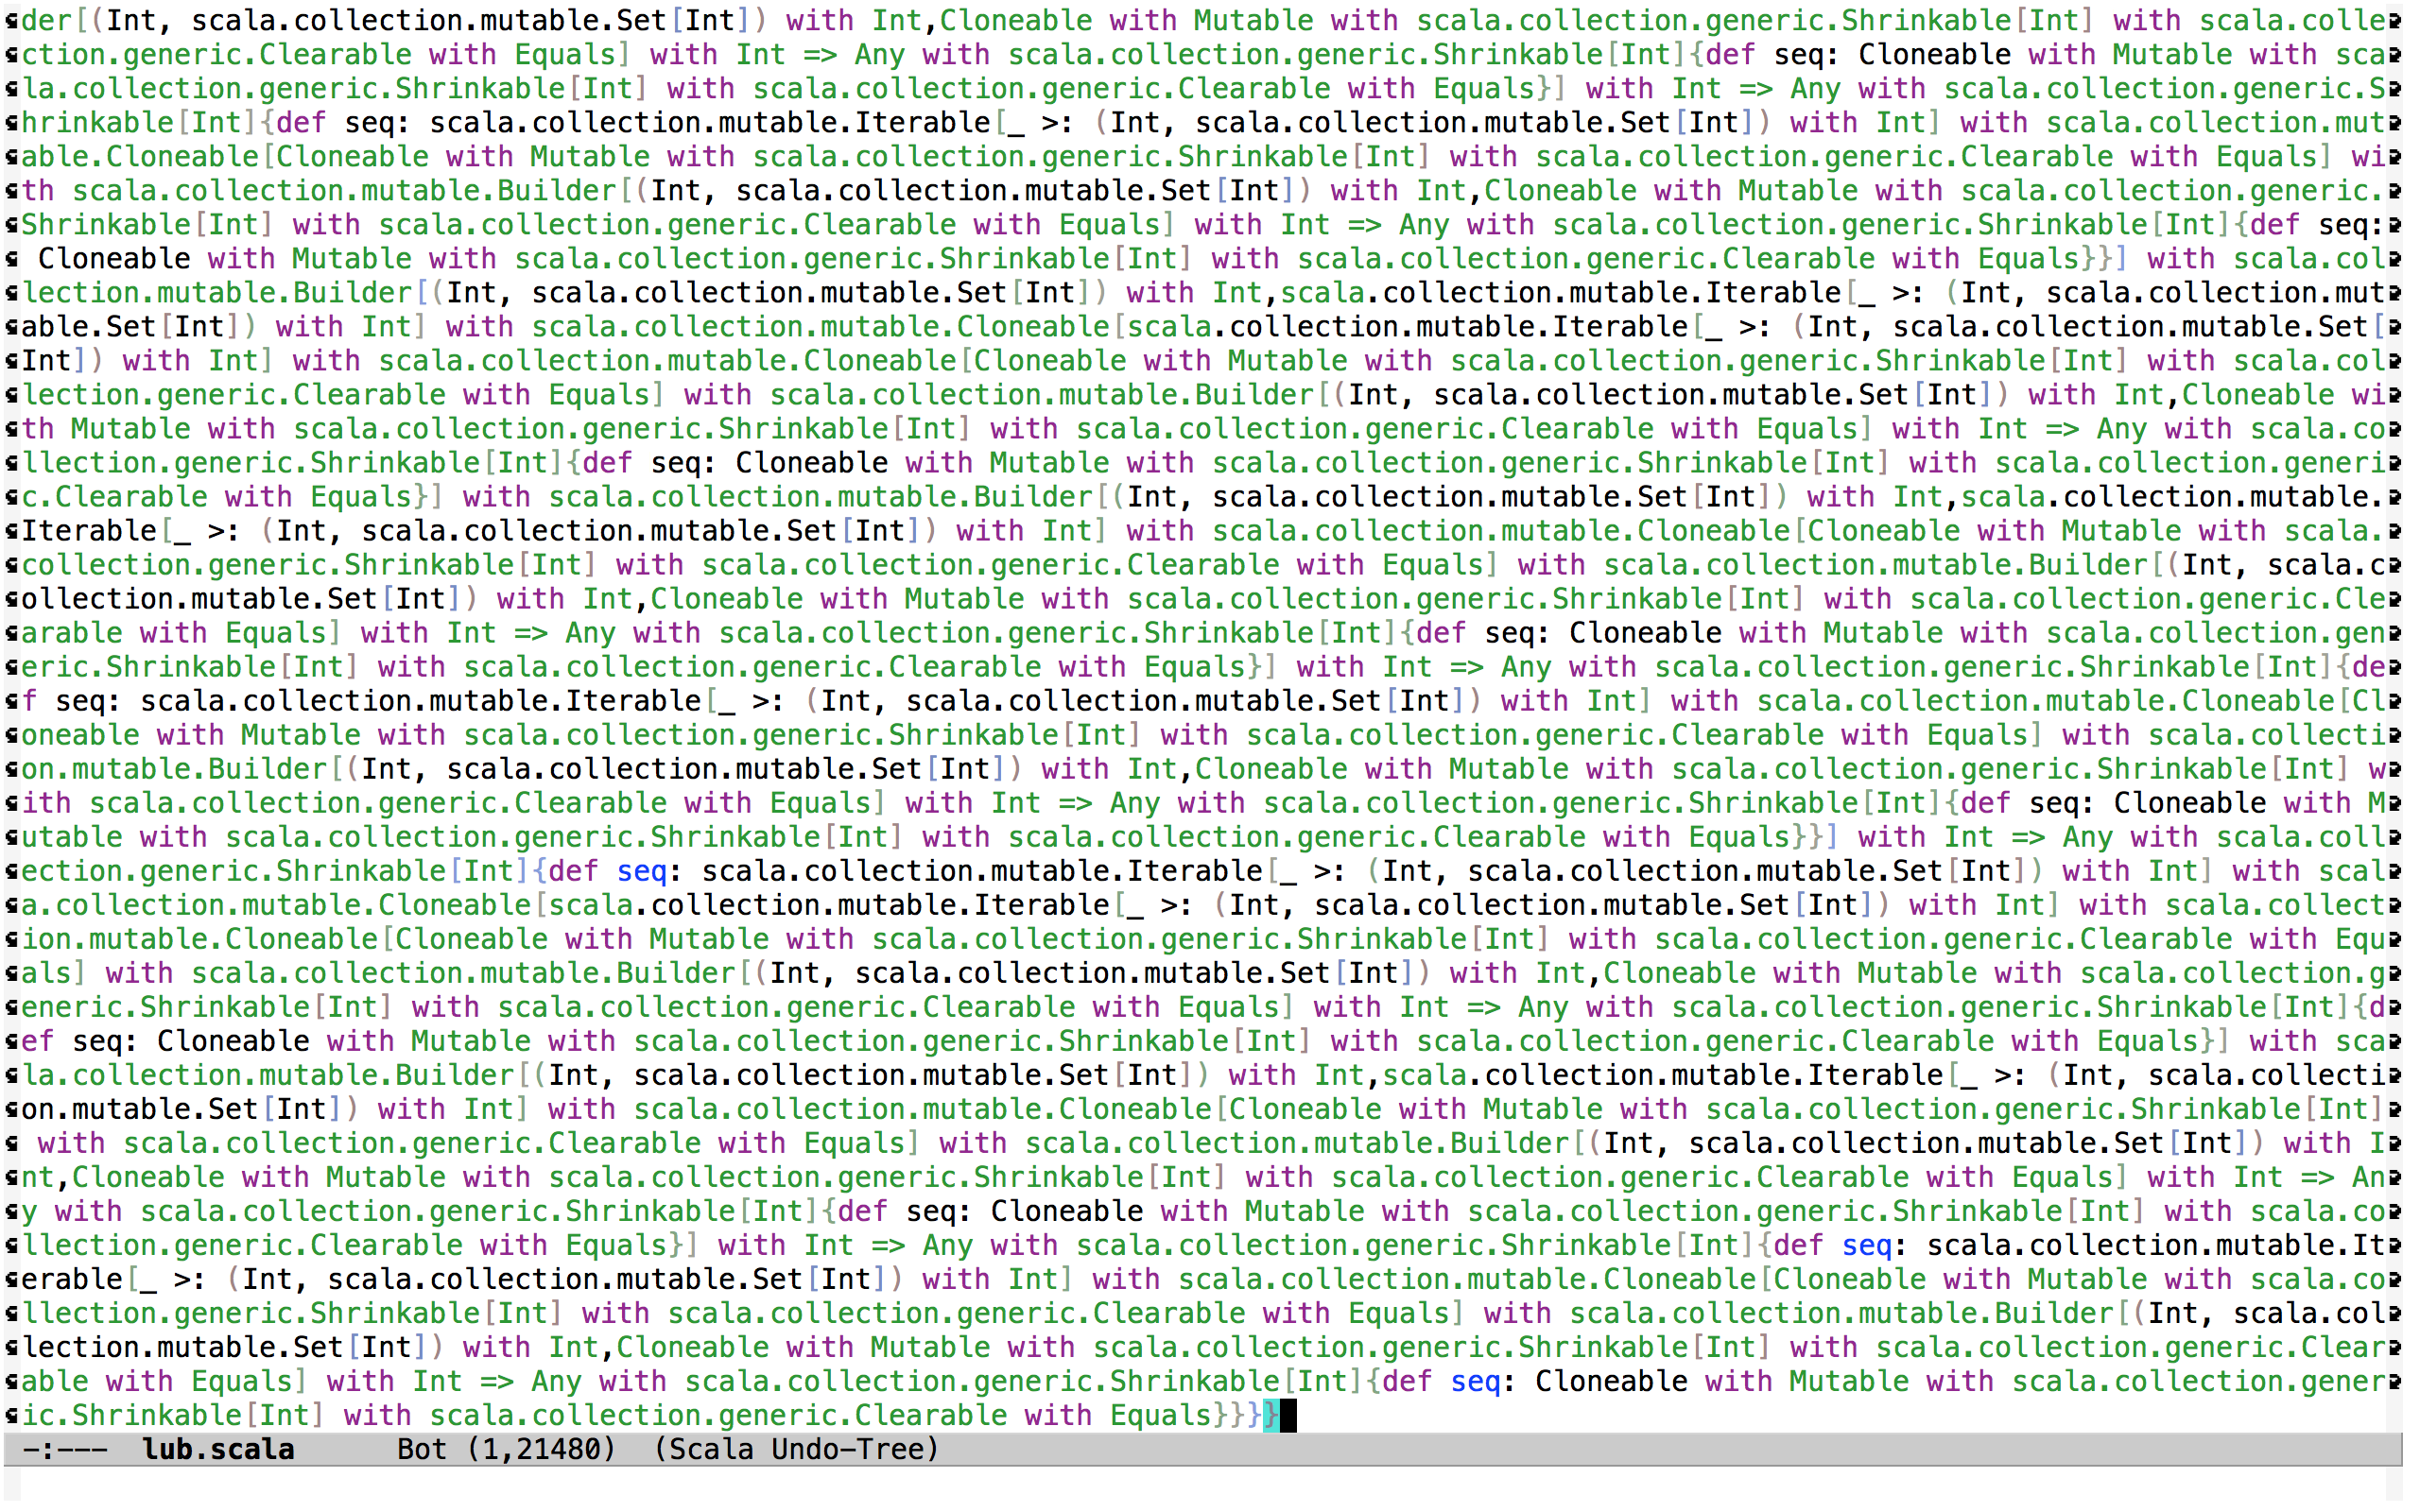
\includegraphics[width=\textwidth]{lub2.png}
\end{frame}

\begin{frame}[fragile]{Type Inference in Scala (Working too Hard too Soon?)}
\begin{minted}{scala}
import scala.collection.mutable.{Map => MMap, Set => MSet}
val ms: MMap[Int, MSet[Int]] = MMap.empty

// in Scala REPL
> if (!ms.contains(1)) ms += 1 -> MSet(1) else ms(1) += 1
res0: ... (796 characters) ...
> :t res0
    : ... (21481 characters) ...
\end{minted}
\begin{itemize}
\item Inspired by a bug report\\
\href{https://issues.scala-lang.org/browse/SI-5862}{SI-5862}: very slow compilation due to humonguous LUB.
\item The character lengths reported are for Scala 2.11 ({\em after} the fix).
\item In Dotty, type inference can be lazy thanks to the native unions (for least upper bounds) and intersections (for greatest lower bounds) of the core calculus (DOT).
\end{itemize}
\end{frame}


\end{document}
